%% This is an example first chapter.  You should put chapter/appendix that you
%% write into a separate file, and add a line \include{yourfilename} to
%% main.tex, where `yourfilename.tex' is the name of the chapter/appendix file.
%% You can process specific files by typing their names in at the 
%% \files=
%% prompt when you run the file main.tex through LaTeX.
\chapter{Technology research} \label{technology_research}

This chapter aims to synthesize the research carried out over the main knowledge areas involved in the development of this project. It intends to give an overview of the technologies and paradigms considered to support the design decisions the project is based upon. Considering the high-level architecture diagram below, these are the main areas of concern initially identified: public interface, that is, the interaction between the sensors and the web server, database, real-time across the system and web technologies.

\begin{figure}[ht]
	\centering
	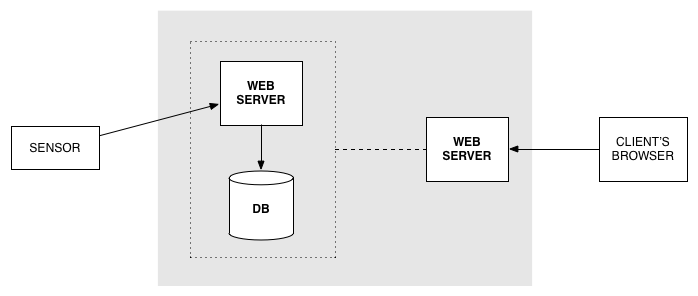
\includegraphics[width=\textwidth]{architecture_analysis}
	\caption{High-level required components}
	\label{fig:arch_analysis}
\end{figure}

\section{Public Interface}

\subsection{Client devices}

In recent years, there has been a steady reduction in costs of hardware devices. Particularly, some microcontrollers have reached prices under 10\$ such as ATmega168, which is the one used by Arduino. Based on a simple microcontroller board and its own development environment, Arduino can be used to develop a vast variety of interactive objects. Its CPU speeds ranging from 8 to 84 Mhz, USB and UART ports, many digital and analog I/O and Flash memory, make it a powerful physical computing device. Even though there are many other affordable microcontroller platforms, Arduino stands out due to its easy-to-use programming environment and cross-platform software. It is especially worth mentioning, however, that this is an open-source physical computing platform. Both its software and the plans of its modules are published under open source licenses.

On the other hand, the decrease in the price of processors for mobile devices with excellent multimedia capabilities led to the foundation of the Raspberry Pi Foundation and the public release of the first Raspberry Pi in 2012. This consists of a single-board computer aimed at teaching computer science basics. Unlike Arduino, it is shipped with 700 MHz ARM processors and as any other computer, it comes with GPU, video and audio outputs and SD storage, but only its Model B has 100 Mbits Ethernet connection. Although it supports some Linux kernel-based operating systems like Debian GNU/Linux and Arch Linux ARM, it is recommendable to run Raspbian, a Debian-based free operating system optimized for the Raspberry Pi hardware. These general purpose features and its credit-card size make it a capable computer which can be used in a wide range of scenarios replacing regular desktop PCs.

Both devices have different aims and capabilities. Arduino is an easy-to-use lower-level physical computing platform, whereas Raspberry Pi beats general purpose PCs in terms of cost and size. Nonetheless, it is not unusual to combine their features attaching them together as a single device, which \cite{Arduberry} attempts. While Arduino brings I/O capabilities that Raspberry Pi lacks, the latter provides computing power.

These features have contributed to their popularity among people involved in technology as well as computing aficionados. They have attracted great interest in the Internet of Things (IoT) community and have had direct impact on its recent growth. Some projects are heavily inspired by Arduino extensibility such as \cite{Thinking-Things}, whilst others build their products based on customized Arduino boards.

This is the case of Smart Citizen \cite{smart-citizen}, a whole platform aimed at generating participatory processes of people in cities thus, creating more effective and optimized relationships between services, technology and communities in the urban environment. The core of the platform is the called Smart Citizen Kit, a hardware device shipped with air, temperature, light, sound and humidity sensors plus a Wi-Fi module to serve as an ambient sensor. They started with Arduino shields to develop a prototype until eventually coming up with their own specific-purpose Arduino-compatible data-processing board.

\subsection{Interoperability} \label{interoperability}

Interoperability is the software quality of enabling a system to interact with other systems without the need to write or maintain custom logic. This is often achieved using the same protocols, exchange or file formats, or by means of standardization.

Interoperability has a great impact on several fields such as financial or medical industries where inadequate implementations may lead to important economic costs. It also crucial in science since the outcomes of a research must be operable for others in order to progress towards a common goal. This also applies in the context of this project since the data obtained by the sensors and its underlying infrastructure may be used in other research projects of CREAF. Not less important is the role this project plays within CREAF's efforts towards the Sensor Web \cite{SWE} as standardization group of the Open Geospatial Consortium (OGC). Therefore, interoperability is a main concern for REDCH.

The OGC's Observations \& Measurements (O\&M) \cite{OM} is the standard data model for storing and publishing sensor data. Based on the Geography Markup Language (GML) OGC standard, it models the relationship between observation events, the spatial objects under observation, the measured properties and measurement procedure and the captured data resulting from the observations. O\&M is one of the open standards developed in the Sensor Web Enablement (SWE) initiative of the OGC.

While O\&M provides a system-independent way of sensor data exchange, the Sensor Observation Service (SOS), another SWE standard, defines a Web service interface for sensor data. This standard allows querying observations and sensor metadata, registering and removing sensors, as well as inserting new sensor observations. Furthermore, it defines KVP and SOAP bindings so as to be binding-independent. However, OGC does not provide an implementation but a service interface.

There are currently some open-source implementations of the SOS. The Earth Science Institute of the University of Applied Sciences of the South Switzerland set up istSOS \cite{istSOS} in 2009, an SOS implementation entirely written in Python that includes a RESTful API and a graphical user interface for easing the administration of the service.

52$\textdegree$North is a network of partners from research, such as the University of Münster and the Technische Universität Dresden, industry, such ESRI Inc. and public administrations such as the IT department of the German Federal Ministry of Transport, Building and Urban Development. It is aimed at bringing innovation into the field of Geoinformatics. 52$\textdegree$North SOS \cite{52north-SOS} is the leading implementation of the Sensor Observation Service. The latest version 4.0, recently released as of this writing, comes with full support of the SOS 2.0 specification. In addition, 52ºNorth has developed the SOS RESTful Extension. A SOS 4.0 Add-on that provides a REST binding beyond the standard KVP and SOAP defined by the OGC.

\section{Database}

The way the data is handled and stored is a key point of the project. Therefore, it is crucial to choose the Database management system (DBMS) that best fits the features of the underlying data set. It must implement some sort of geographic support as every observation implicitly belongs to a particular geographic location.

Databases allow to persist a representation of real-world objects and their relations in a structured fashion. Furthermore, they also allow to integrate the data of different applications thus, avoiding data duplication.

Databases may be classified in three general models: hierarchical, network, relational and NoSQL. Relational databases have gained a lot of popularity since their appearance in the late 1970s, becoming the de facto choice regarding data management in IT systems. On the ohter hand, NoSQL systems is a field that has been quickly evolving very fast since its birth in the 2000s.

\subsection{Relational DBMSs}

The relational model is based on set theory and predicate logic. Relational databases implement an approximation of these mathematical models using a table-based format. The data is structured in tables that represent relations where the information of a particular entity is represented by a row and the set of fixed attributes of such entity correspond to the columns.

Databases, however, need DBMSs in order to be functional. A DBMS is an especially designed software which enables the creation, querying, update, and management of databases. It is a layer above the OS that abstracts the applications from the database. Hence, applications deal with databases through the DBMS.

Relational DBMSs essentially provide efficient, reliable, convenient, and safe multi-user storage of and access to massive amounts of persistent data. These guarantee consistency by means of robust concurrency models and ACID (Atomicity, Consistency, Isolation, Durability) transactions. Due to decades of development and research relational database systems are relied upon by mission-critical applications that demand strict consistency.

The most popular open-source relational DBMSs are MySQL and PostgreSQL, both with spatial extensions. PostGIS, however, is the most mature solution. It is a PostgreSQL extension that adds support for location awareness enabling queries by geographic location. In addition, PostGIS supports geographic coordinates. As a consequence of PostGIS' rich feature list, PostgreSQL is the standard choice for Geographic Information Systems (GIS).

However, not every data management or analysis problem is best solved exclusively using a traditional DBMS. There are some problems that are more suitable for other type of systems \cite{NoSQL-use-cases}.

\subsection{NoSQL Systems}

NoSQL Systems, whose name stands for \textit{Not Only SQL}, differ from traditional relational systems in that they tend to provide a flexible schema rather than a rigid structure. They are also quicker and cheaper to set up geared towards massive scalability and use relaxed consistency in order to provide higher performance and higher availability.

Their downsides are that there is no declarative query language thus, more programming is involved in manipulating the data. Furthermore, because of the relaxed consistency models, their better performance comes at the expense of fewer guarantees about the consistency of the data. Eventually consistent systems are often classified as providing BASE (Basically Available, Soft state, Eventual consistency) properties in contrast to traditional ACID-compliant relational systems.

One of the main goals of NoSQL systems is to enhance horizontal scalability. As the CAP theorem states \cite{CAP-theorem}\cite{CAP:online}, this can only be achieved by relaxing either its consistency or its availability so partition tolerance may be guaranteed. There is no consensus among NoSQL vendors over which pair to choose. Some opt for consistency against availability, while others focus on availability over consistency \cite{CAP-NoSQL}. Nonetheless, there are few that pick both properties and consequently provide scalability through replication rather than partitioning.

The number of different kinds of NoSQL systems may be generalized in four main categories: MapReduce frameworks, Key-value stores, Graph database systems and Document stores. MapReduce frameworks are typically used in applications that process large amounts of data to do complex analysis, whereas Key-value stores tend to perform a lot of small operations on very small parts of the data. On the other hand, Graph database systems are designed for storing and operating over very large graphs.

\paragraph{Document stores}

Document stores are very similar to Key-value stores except that the values are documents. Hence, the data model is based on ${<key, document>}$ pairs where the document is a known type of structure that can contain semistructured data formats such as JSON or XML. Like in key-value stores the basic operations allow a document to be fetched, updated, deleted and inserted based on a given key. Additionally, they also implement a fetch operation based on document contents which is a very implementation-specific feature since there is no standard query language. Few examples of document stores are CouchDB, MongoDB and Amazon's SimpleDB, among many others.  

In addition, MongoDB, CouchDB and SimpleGEO support geospatial indexing allowing to query for location-based data. Although not as accurate as PostGIS, these NoSQL systems may fit in some use cases where performance and scalability are critical.

\section{Real-Time in Distributed Systems}

As defined in \cite{distributed-systems-book} a distributed system is \textit{a collection of independent computers that appears to its users as a single coherent system}. This involves some sort of collaboration between the autonomous components (i.e., computers). Although discussing the advantages and disadvantages is not the topic of this writing, the main benefits of distributed architectures over centralized systems are the greater scalability, improved resilience and higher availability. To do so, distributed systems decouple a single application in a number of components that handle the diverse functionalities of the whole system. This enables the horizontally scaling in an independent way and makes them fail-tolerant. However, this impose other problems as the components need to share state and communicate. Moreover, failure-handling is often a complex task. \cite{DT-fallacies} presents a summary of the main distributed computing concerns.

The challenge that real-time in a distributed environment entails is essentially the management of the system's state, as happens with non-real-time distributed systems. Particularly, real time systems are systems in which the timeliness of the operations is a part of the functional requirements and correctness of the system. However, nearly all systems may be qualified as \textit{soft} real-time, in that there are usually unspoken expectations for the timeliness of operations.

On the other hand, \textit{hard} real-time refers to systems which don't fulfil the requirements when time constraints are not met. This kind of systems are commonly known as Distributed Real-Time systems.

\subsection{Message Passing} \label{message_passing}

Instead of sharing the memory, in distributed systems is generally a better approach to share state by communicating. Message passing is a communication model that involves calling a subroutine by sending a message to an intermediary process. It relies on its infrastructure to invoke the actual code rather than calling subroutine by name as in a traditional procedure call. In such systems, communication is explicit and functions are separated from the specific implementations. (Immediate drawbacks)

An immediate upside of such communication model is the loose coupling between components. With a remote procedure call, the sender process must know the receiver and the complete signature of its procedures beforehand whereas with message passing, sender and receiver are nearly independent. This allows the system's components to be upgraded one at a time, thus giving the system the ability to evolve. Furthermore, it also improves interoperability. If the message is text-based (i.e., JSON, XML) there is no requirement for the components to be built in the same platform, operating system or language.

As all information regarding the state is contained in the messages there is no need for the receiver to store state information thus providing statelessness to the system. Although it comes at the cost of a slightly longer transmission time, this drastically improves the system's scalability.

Message passing systems are categorized in two main groups whether they implement synchronous or asynchronous messaging. In the former, the sender and the receiver must be running at the same time for the message to be passed while in the latter the receiver is not required to be running at the time the sender sends the message. As a consequence, asynchronous messaging requires additional data storing and retransmitting capabilities for components that may not run concurrently.

In regular function calls, the caller waits for the called function to complete. Likewise, in synchronous message passing the sending process remains blocked until the receiving process finishes. The resulting impact on performance is generally unaffordable for large distributed systems, particularly for those with hard real-time constraints.

In contrast, asynchronous messaging is non-blocking. The sending process delivers the function call along with any needed arguments wrapped in a message to the message layer and continues its execution thread. The message layer acts as a intermediary between sender and receiver and so is considered a middleware. It stores the message until the receiver requests messages sent to it. Then, the receiver sends a message back with the result and the message layer stores it until the sender fetches its messages. Asynchronous messaging software is often referred to as Message Queues. Essentially, messaging middlewares store messages in a queue and processes them in a FIFO fashion.

Besides commercial products of well-known vendors such as Oracle or IBM, there are many open-source queueing systems available \cite{queues} due to the standardization of AMQP and STOMP protocols. As a consequence, there is no restriction for different programming languages to interact with queueing systems based on these standards. Each one of these has been created for solving specific problems.

The most widely popular and successful running on production systems are Apollo, HornetQ, RabbitMQ and ZeroMQ. The first one is a major rewrite of the Apache's ActiveMQ with better reliability and performance. It is an implementation of the Java Message Service (JMS) specification with support for Enterprise Integration Pattern required for distributed transactions. It supports STOMP, AMQP, MQTT, OpenWire and WebSockets plus SSL support. Additionally, Apollo also provides a REST Management API.

HornetQ is fully JMS 1.1 compliant, previously integrated in the JBoss Application Server under the name of JBoss Messaging 2.0. Although further developed as a separated project, it provides seamless integration into JBoss. It is focused on reliability and contains lots of features and configurable settings at the expense of a certain degree of complexity. Its REST interface allows it to be used by any programming language, besides the HornetQ client libraries available.

RabbitMQ, written in Erlang, is specially suited for high performance distributed applications with great support for concurrency, availability and clustering. With its core fully supporting the AMQP protocol, it can understand STOMP protocol as well through its plug-in architecture. Furthermore, there are client libraries available for multiple languages and integrations with popular frameworks. Finally, its management plugin provides a web console that allows easy administration and detailed resources monitoring.

ZeroMQ, on the other hand, provides a library to create distributed and concurrent applications rather than a message queue. In contrast to the aforementioned message-oriented middlewares, ZeroMQ doesn't require a central server. The sender process handles the routing and the receiver deals with the queueing. This approach enables very low latency and high throughput resulting in substantially better performance. Therefore, it's ideal for large volume of messages like in financial transactions or online games.

It is worth mentioning, however, the MQ Telemetry Transport (MQTT) a pub/sub, simple and lightweight messaging protocol, designed for constrained devices and low-bandwidth, high-latency or unreliable networks. It is fully geared towards the minimisation of network bandwidth and device resource, over reliability and resilience. Therefore, it is especially suitable for the Internet of Things, the sensor web and mobile applications.

Scalability and reliability don't make a difference between all the above products, except for MQTT, as all of them are highly scalable, robust and reliable. With regards to performance, it's really difficult to objectively evaluate even with standardized benchmarks. However, as already stated, ZeroMQ is by far the most performant message queue when message persistence is not required. Althought there's not much difference between other solutions, RabbitMQ tends to beat others when used with AMQP protocol.

\section{Web Technologies}

Since the Sir Tim Berners-Lee's first draft of the World Wide Web back in 1989 and his first proposal for the HyperText Markup Language (HTML) \cite{HTMLtags} in 1991 the WWW has experienced a tremendous evolution. Since then, HTML has gone through many revisions. The World Wide Web Consortium (W3C) published many iterations of the standard until the specification HTML 4.01 in 1999. It was not until 2004, when the Web Hypertext Application Technology Working Group (WHATWG) was founded to extend HTML so as to allow the creation of web applications. WHATWG published the First Public Working Draft of the HTML5 specification in 2008. Although parts of HTML5 have already been implemented in browsers, it was not until 2012 that W3C designated HTML5 as a Candidate Recommendation. It is scheduled for release as a stable Recommendation by the end of 2014.

\subsection{HTML5}

HTML5 is designed to deliver rich content without the need for third-party plugins while being backward compatible. As happened in HTML 4.01 with CSS 1.0, in HTML5 JavaScript is an integral part of the specification along with CSS3. The standard defines multiple JavaScript APIs such as drag and drop, files, webRTC, audio and video, webGL, etc. while others like vibration or accelerometer APIs are still in development.

HTML5 together with XMLHttpRequest API, the technology behind AJAX, already present in major browsers some years ago, has turned web browsers into web application containers. This fact has stimulated the development of JavaScript libraries. Some try to solve cross-browser issues like jQuery. Since its creation in 2006 it has become the standard for manipulating the DOM and for dealing with AJAX requests due to its simplicity and extensibility.

As for JavaScript frameworks, there is a myriad of choices due to the rebirth of the JavaScript community over the last few years. These modern JavaScript frameworks like Backbone.js, Ember.js, AngularJS, CanJS and others provide structure, organization and maintainability to the so called single-page applications (SPA). All of them implement variations of the Model-View-Controller (MVC) pattern.

Much like jQuery improved the DOM manipulation, D3.js happens to be essential as well when it comes to data visualizations. Its concepts provide an abstraction layer that enables the manipulation of documents based on data. It converts data to visualizations using HTML, SVG and CSS with lots of features through a large collection of components and plugins. It is worth mentioning its geographic projections along with layouts and geometry plugins which may come in handy in our project and its further development.

\subsection{Real-Time} \label{web_real_time}

The web follows the pull paradigm by design. In HTTP, communication is initiated by the client who sends a request to a server. The server then sends a response back to the client. That is, the client pulls data from the server. While this approach works fine for fetching documents from a server, for which the web was initially designed, it does not work when the server needs to initiate the communication.

The first and most common solution to this issue is what is known as polling, that is, to request information from the server at regular intervals regardless of whether it has new data available. A further improvement of this approach is to make these requests wait until new data available, which is called long polling or comet. Both techniques, however, entail a waste of resources and are clearly non-real-time.

Nonetheless, HTML5 has provided two new techniques to solve this common issue and bring push capabilities to the web. Server Sent Events (SSE) is a W3C specification \cite{SSE} that defines an API for opening an HTTP connection for receiving push notifications from a server through a half-duplex channel. It is designed to be extended to work with other notification schemes such as SMS. Furthermore, it has features like automatic reconnection, event identifiers and the ability to send custom events.

With server-sent events, it's possible for a web server to send data to a web page at any time by pushing messages into it. The client initiates the communication by issuing a request to the server when a new EventSource object is instantiated in JavaScript. Then the server pushes the messages as DOM events that can be listened to like any other JavaScript event source.

On the other hand, WebSockets provide a richer protocol with support for bi-directional, full-duplex communication. They have drawn much more attention than server-sent events due to its richer feature set. WebSockets is a TCP-based protocol \cite{WS} completely separate from HTTP that provides low-latency two-way communication for browser-based applications.

Its bidirectional capabilities makes it particularly suitable for games, messaging apps and for use cases where near real-time updates in both directions is needed. Additionally, it provides cross origin communication, which enables communication between parties on any domain. As a downside, since it's not HTTP it requires specific infrastructure such as a server enabled to deal with this protocol.
